%==============================================================================
% Capitulo 5: Arquitectura del Sistema
%==============================================================================
\section{Arquitectura del sistema}

\subsection{Visión general}

El sistema propuesto se estructura como una arquitectura distribuida y modular compuesta por cinco capas claramente diferenciadas, siguiendo los principios de cohesion alta y acoplamiento bajo descritos por \textcite{Pressman2020_software_engineering}. En el diseño se previó proteger la comunicación con el exterior mediante TLS~1.2/1.3 a nivel de un proxy inverso (Nginx); el despliegue publicado para la validación experimental no incluyó dicho proxy, por lo que la terminación TLS corresponde al diseño y no a una capacidad verificada en la instancia publicada. La comunicación interna entre los servicios del sistema (N8N, backend, PostgreSQL, Redis) se realiza sobre la red aislada de Docker, que constituye el perímetro de confianza. Todas las interfaces entre capas utilizan el estilo arquitectónico REST con cuerpos JSON para el intercambio estructurado de datos \parencite{Fielding2002_rest}. Esta separación de responsabilidades facilita el reemplazo independiente de cualquier componente sin afectar a los demas.

La Tabla~\ref{tab:capas} sintetiza las cinco capas y sus responsabilidades específicas.

\begin{table}[htbp]
\centering
\caption{Capas funcionales de la arquitectura del sistema}
\label{tab:capas}
\small
\begin{tabular}{@{}>{\raggedright\arraybackslash}p{3.0cm} >{\raggedright\arraybackslash}p{10.5cm}@{}}
\toprule
\textbf{Capa} & \textbf{Componentes y responsabilidades} \\
\midrule
1. Canales de entrada & Casilla de correo electrónico monitoreada mediante IMAP/SMTP, formulario web implementado como SPA React y número virtual de Twilio con transcripción automática del habla. \\
2. Orquestacion & Motor N8N~2.11.2 desplegado en contenedor Docker autoalojado. Normaliza la entrada y coordina la invocacion a las capas inferiores. \\
3. Procesamiento & Servicio Python sobre FastAPI~0.115 ejecutado bajo Uvicorn. Aplica clasificador hibrido en dos etapas (reglas + LLM) y expone una API REST documentada con OpenAPI~3.1. \\
4. Inferencia & Modelo Gemini~3.6 Flash de Google, invocado únicamente cuando el filtro deterministico previo no alcanza el umbral de confianza preestablecido. \\
5. Persistencia & PostgreSQL~15.5 desplegado en contenedor con volumen persistente y respaldos diarios. Almacena los incidentes y la trazabilidad de cada decision del clasificador. \\
\bottomrule
\end{tabular}
\par\smallskip
{\footnotesize\textit{Fuente:} elaboración propia.\par}
\end{table}

La trazabilidad operativa se garantiza mediante registros estructurados en cada capa, accesibles desde la capa de orquestación. La Figura~\ref{fig:arquitectura} representa esquematicamente el flujo de información entre capas.

\begin{figure}[htbp]
\centering
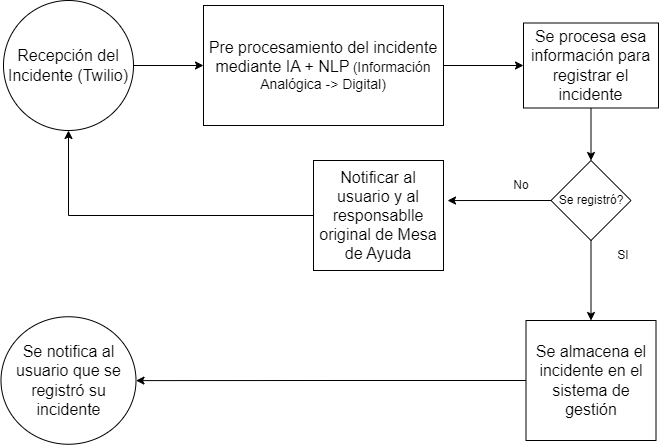
\includegraphics[width=\textwidth]{arquitectura_sistema}
\caption{Diagrama de arquitectura del sistema. La version completa en notacion UML se incluye en el Anexo~A.}
\label{fig:arquitectura}
\end{figure}

\begin{figure}[htbp]
\centering
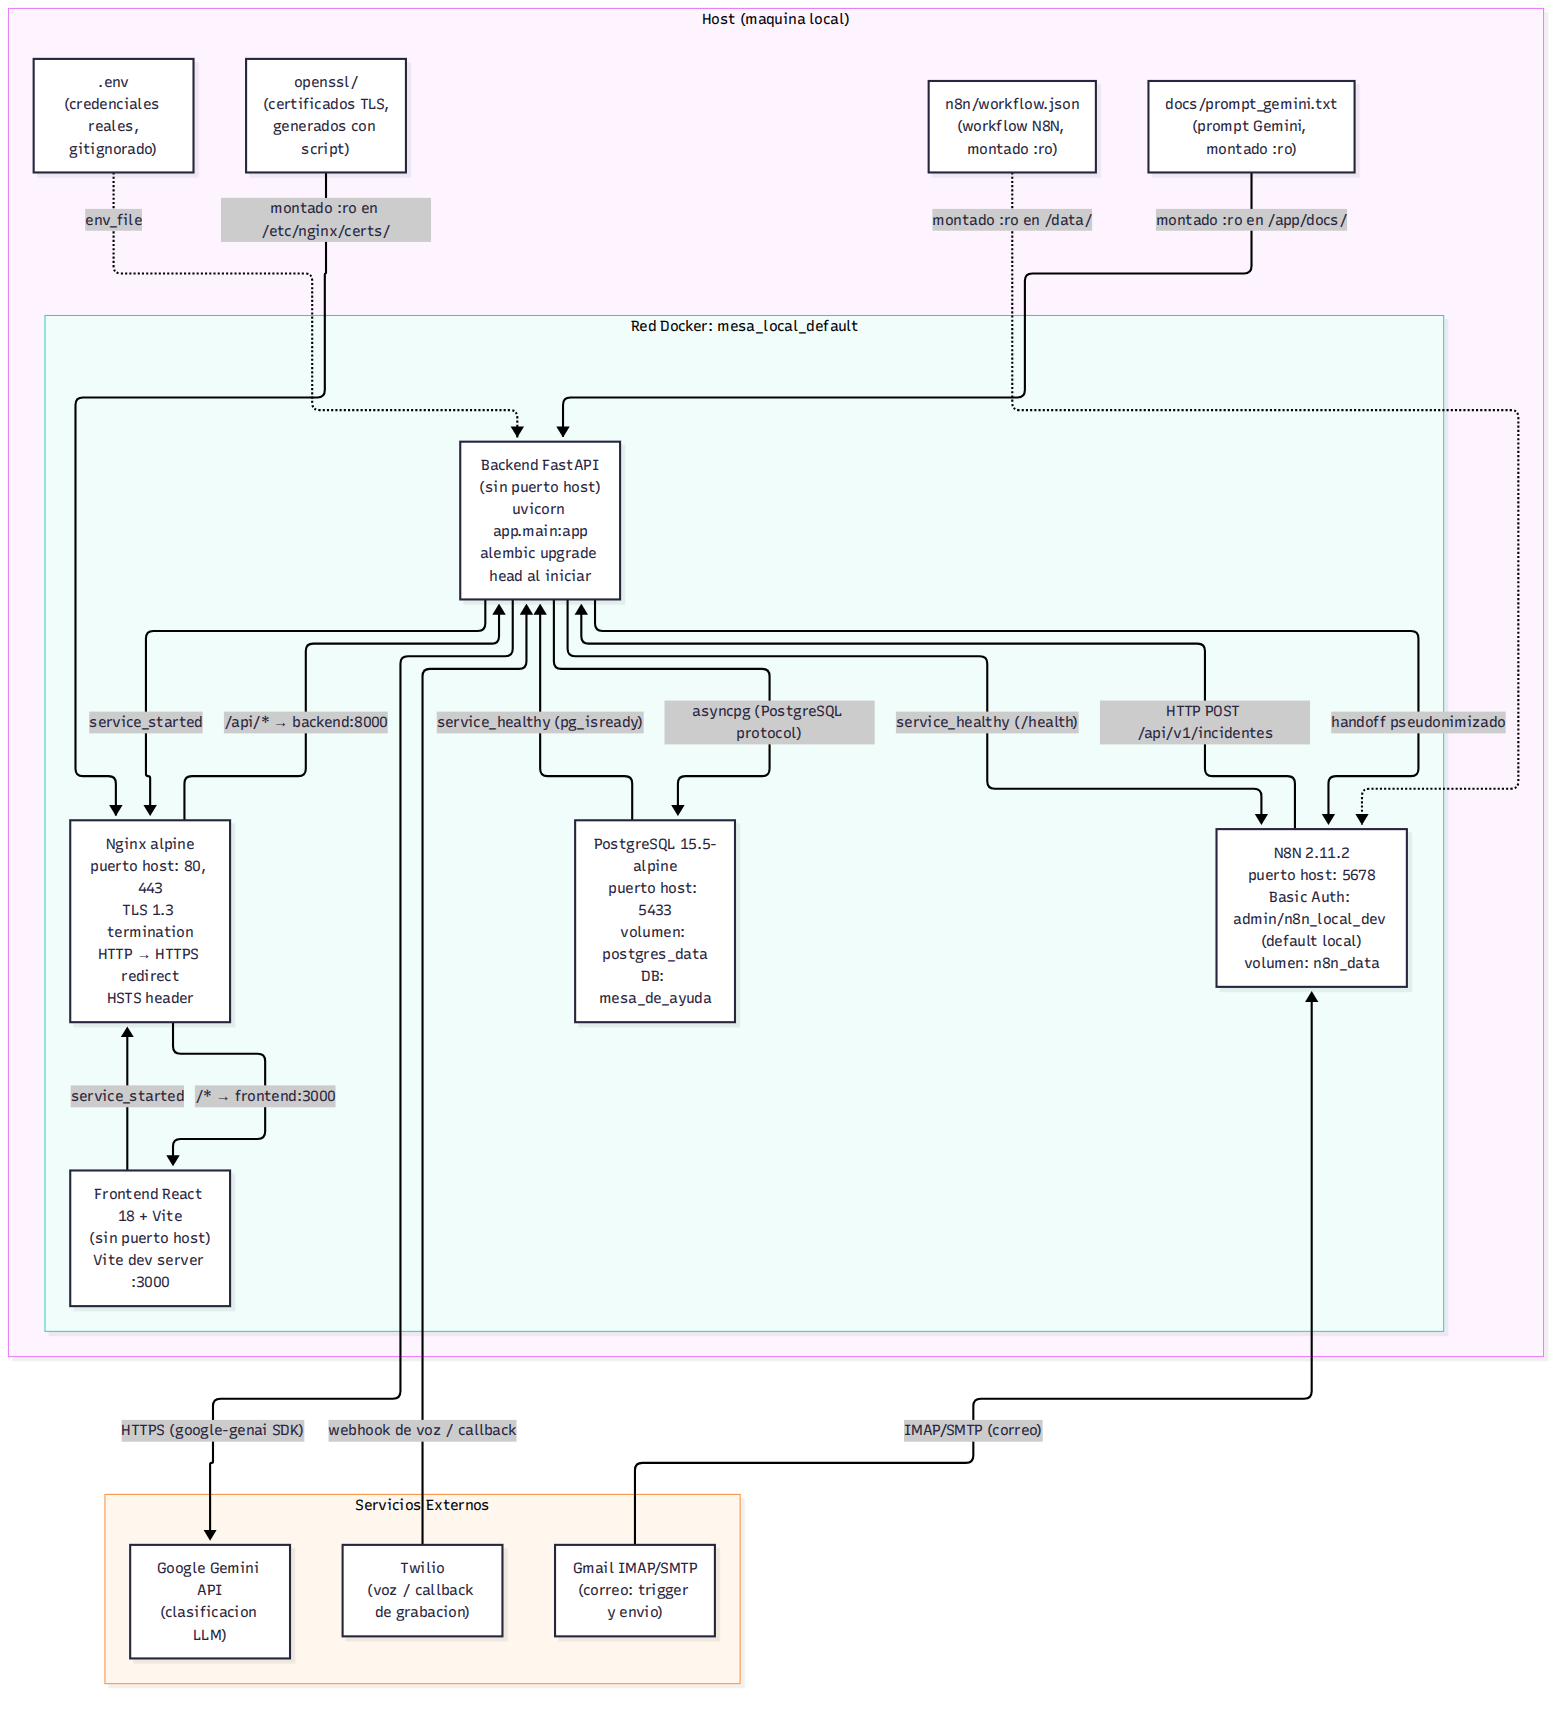
\includegraphics[width=0.92\textwidth]{despliegue}
\caption{Diagrama de despliegue del entorno local. Servicios, red Docker, volumenes y servicios externos.}
\label{fig:despliegue}
\end{figure}

\begin{figure}[htbp]
\centering
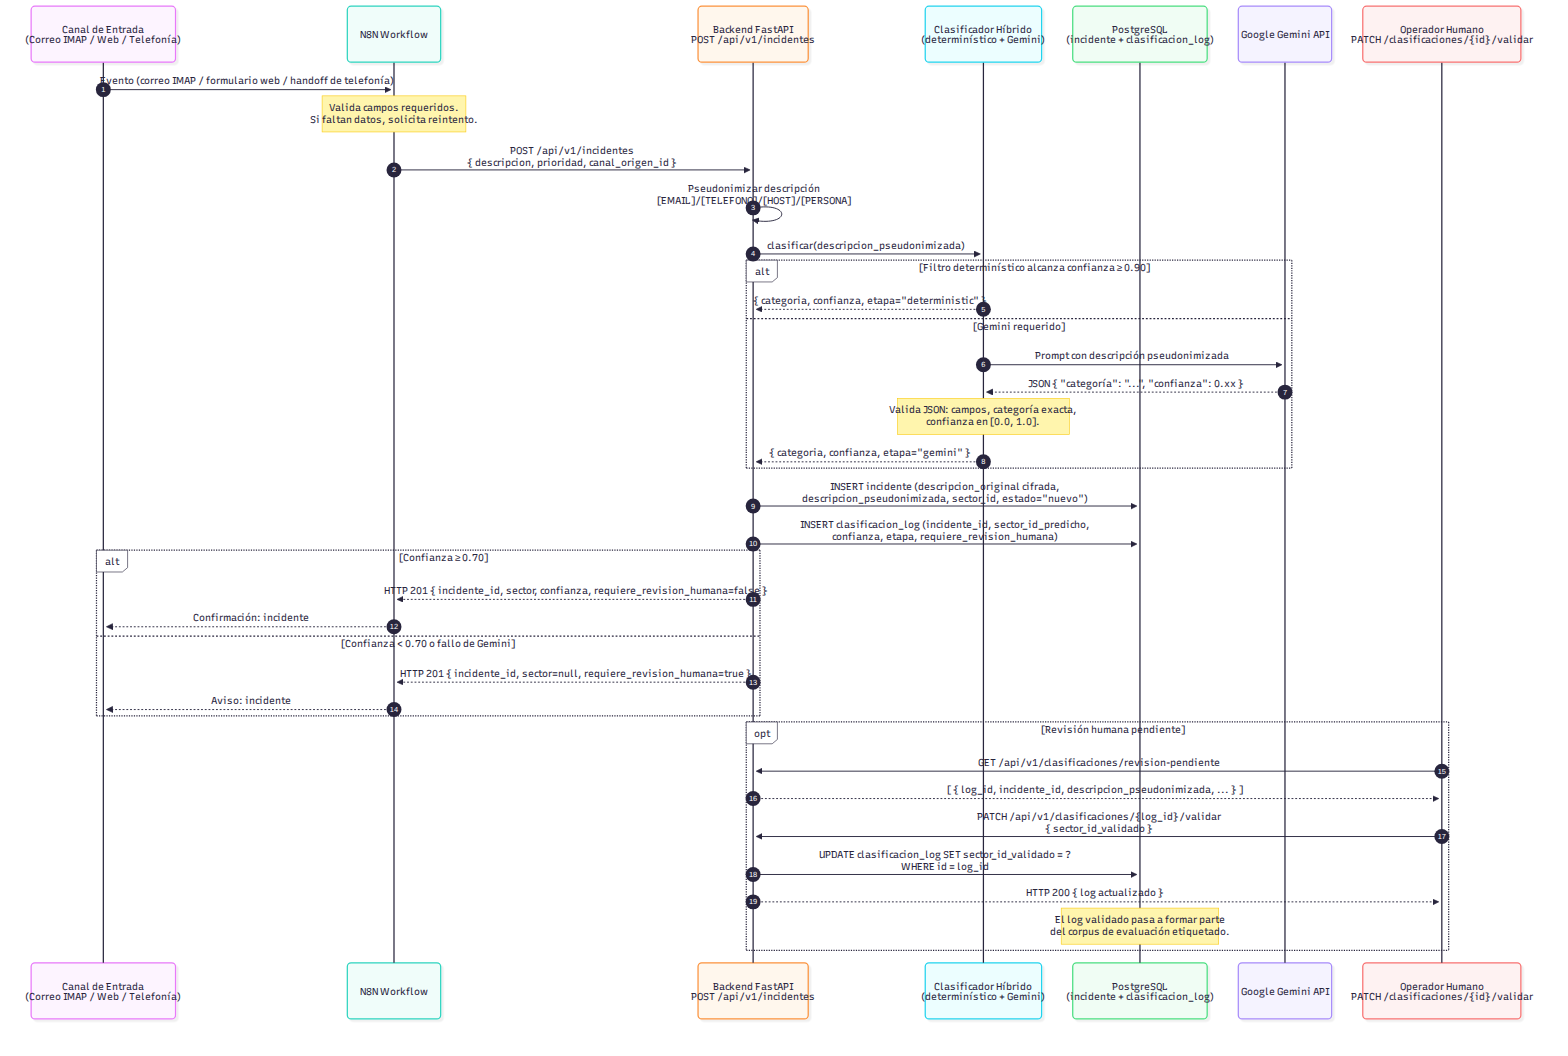
\includegraphics[width=\textwidth]{secuencia}
\caption{Diagrama de secuencia del flujo extremo a extremo de un incidente, desde el canal de entrada hasta la confirmacion o la derivacion a revision humana.}
\label{fig:secuencia}
\end{figure}

\subsection{Capa de canales de entrada}

La capa de canales de entrada habilita tres vias paralelas a través de las cuales un usuario puede reportar un incidente. La primera es el correo electrónico, monitoreado mediante IMAP/SMTP que detecta nuevos mensajes en una casilla institucional dedicada. La segunda via es un formulario web implementado como aplicación React de página única (SPA) que se comunica directamente con la API REST del módulo de procesamiento. La autenticación se realiza mediante tokens JWT (JSON Web Tokens) con usuario y contraseña; la autenticación única corporativa (SSO) se prevé como evolución para entornos productivos (Capítulo 10). La tercera via es la llamada telefónica, en la cual el usuario marca un número virtual provisto por Twilio, recibe instrucciones por voz pregrabadas y deja su solicitud; la grabación es transcrita automáticamente por el servicio de reconocimiento del habla del proveedor y enviada al flujo N8N mediante webhook posterior al cuelgue. El script TwiML que define el flujo de la llamada —incluyendo el mensaje de bienvenida en español rioplatense y la configuración de grabación— se encuentra documentado en el Anexo~E. Esta diversidad de canales amplía la accesibilidad del sistema y reduce las barreras al reporte oportuno.

\subsection{Capa de orquestación}

N8N actua como orquestador principal del flujo de trabajo: recibe la entrada de cada canal, la normaliza en una estructura unificada y coordina la clasificación y la persistencia del incidente. La descripción operativa detallada del flujo ---los disparadores por canal, la estructura normalizada con identificador único (UUID v4), la invocación al modulo Python y la persistencia del ticket--- se desarrolla en la Sección~6.3. Los registros de cada ejecución se conservan durante 30 días para fines de auditoria y diagnostico operativo; constituyen un conjunto de datos distinto de los incidentes, cuya retención se rige por la política declarada en la Sección~11.2.

\subsection{Capa de procesamiento}

El modulo de procesamiento se implementó como un servicio web ligero utilizando el marco FastAPI~0.115, expuesto sobre un servidor ASGI Uvicorn 0.30.6 \parencite{Tiangolo2024_fastapi}. La eleccion de FastAPI obedece a su soporte nativo de validación de esquemas mediante Pydantic, su rendimiento competitivo y su documentación automática conforme a la especificación OpenAPI~3.1.

Las dependencias del modulo se organizan por capas funcionales claramente delimitadas. La capa de acceso a datos utiliza SQLAlchemy~2.0 como mapeador objeto-relacional (ORM) y asyncpg como driver asincrónico para PostgreSQL, en coherencia con la operación no bloqueante de FastAPI. La capa de procesamiento textual emplea las bibliotecas regex y unicodedata de la biblioteca estandar de Python para normalización ortografica y eliminacion de signos diacriticos. La capa de inferencia se comunica con la interfaz oficial del modelo \texttt{gemini-3.6-flash} mediante el cliente google-genai >=2.0 (SDK unificado de Google Generative AI), con los siguientes parámetros de configuración: temperatura \(= 0{,}3\), top\_p \(= 0{,}9\), max\_tokens \(= 100\) y timeout \(= 10\)~s. Estos valores corresponden a la configuración adoptada para el despliegue y no a un procedimiento de optimización documentado; su calibración sistemática frente a valores alternativos se plantea como trabajo futuro (Capítulo~10). Las bibliotecas NumPy~2.1 y Pandas~2.2 se utilizan exclusivamente para la generación de reportes agregados de desempeño y no participan del flujo de procesamiento individual de incidentes.

\subsection{Subsistema de clasificación híbrido}

El subsistema de clasificación adopta un enfoque hibrido en dos etapas, caracteristica que lo diferencia de aproximaciones puramente basadas en modelo externo. La primera etapa aplica un filtro deterministico basado en expresiones regulares y diccionarios de terminos del dominio. Para mitigar el riesgo de fuga de datos (\emph{data leakage}), la construcción del filtro deterministico se realizó de forma rigurosa: primero, se definieron manualmente un conjunto de patrones regex basados en conocimiento del dominio y análisis preliminar de descripciones de incidentes (análisis que no utilizó el corpus de validación de 200 casos); segundo, los parámetros del prompt enviado a Gemini~3.6 Flash se ajustaron exclusivamente mediante validación manual sobre incidentes representativos en entornos de preproduccion, sin acceso al corpus de validación.

Este filtro es capaz de derivar de forma inmediata aquellos incidentes que contienen marcadores inequivocos. Por ejemplo, la presencia simultanea de las palabras \texttt{impresora}, \texttt{papel} y \texttt{atasco} sugiere con alta certeza una categoría de Soporte Tecnico. Cuando este filtro inicial alcanza un umbral de confianza superior al 90~\%, la decision se toma sin consultar al modelo externo, lo que reduce sustancialmente la latencia y el costo de inferencia.

La segunda etapa, activada únicamente cuando el filtro deterministico no alcanza el umbral, consulta al modelo Gemini~3.6 Flash mediante un prompt estructurado en espanol que incluye una breve descripción de cada categoría, ejemplos representativos balanceados y la solicitud explicita de devolver la categoría asignada y un valor numerico de confianza entre 0 y 1 en formato JSON estricto. La justificación de este diseño compositivo radica en aprovechar la rapidez del filtro deterministico para los casos triviales y reservar la capacidad semántica del modelo de lenguaje grande para los casos ambiguos o de redacción atipica, optimizando la relacion entre exactitud, costo y latencia. El pipeline completo comprende tres etapas, aplicadas en orden: (1)~el filtro deterministico, (2)~el modelo Gemini y (3)~una etapa de reserva (\emph{fallback}) que asigna una categoría por defecto y marca el caso para revisión humana cuando las etapas previas no producen una salida válida. La medición sobre el corpus de validación muestra que la etapa determinística resolvió 131 de los 200 casos (65,5~\%), la etapa Gemini 69 casos (34,5~\%) y la etapa de reserva no se activó en ningún caso (0 de 200).

El camino de clasificación es único para los tres canales de entrada. Tanto el correo electrónico y el formulario web como la llamada telefónica resuelven su sector mediante esta misma cascada híbrida, aplicada sobre la descripción pseudonimizada del incidente: ningún canal aporta una clasificación precalculada que omita la cascada, de modo que las reglas determinísticas, el prompt y las reglas de frontera se ajustan una sola vez para todo el sistema. El prompt único incorpora reglas de desambiguación de frontera entre sectores adyacentes (acceder o iniciar sesión en una aplicación se orienta a Soporte Tecnico Software; la digitalización, el escaner o la impresora se orientan a Soporte Tecnico Hardware; el servidor, la red, SMTP o una VM se orientan a Sistemas), redactadas con los cinco strings canónicos sin tildes. Desde el punto de vista del costo, la clasificación telefónica dejó de computarse sobre una invocación incondicional al modelo externo: el canal atraviesa el filtro determinístico y solo escala al modelo semántico cuando la cascada lo requiere, momento en el cual la reserva de costo se imputa a la superficie de inferencia del backend.

\subsection{Modelo de datos}

La persistencia se realiza sobre PostgreSQL~15.5, desplegado en contenedor Docker bajo configuración de respaldo diario y replicación fisica opcional para entornos productivos \parencite{PostgreSQL2024_docs}. El modelo de datos se organiza alrededor de siete entidades principales, descritas en la Tabla~\ref{tab:entidades}.

\begin{table}[htbp]
\centering
\caption{Entidades principales del modelo de datos}
\label{tab:entidades}
\small
\begin{tabular}{@{}p{2.5cm} >{\raggedright\arraybackslash}p{4.8cm} >{\raggedright\arraybackslash}p{5.5cm}@{}}
\toprule
\textbf{Tabla} & \textbf{Atributos clave} & \textbf{Descripcion} \\
\midrule
\texttt{incidente} & id\_incidente (PK), canal\_origen\_id (FK), id\_sector (FK), id\_estado (FK) & Tabla central: fecha de creacion, descripción cruda pseudonimizada, prioridad, sector asignado y estado actual. \\
\texttt{sector} & id\_sector (PK), nombre & Catalogo de los cinco sectores canónicos: Seguridad Informática, Soporte Técnico Hardware, Soporte Técnico Software, Bases de Datos y Sistemas. \\
\texttt{estado} & id\_estado (PK), nombre & Catalogo de estados: nuevo, en proceso, en espera, resuelto y cerrado. \\
\texttt{canal\_origen} & id (PK), nombre & Catalogo de canales: correo, formulario web y llamada telefonica. \\
\texttt{clasificacion\_log} & id\_log (PK), id\_incidente (FK), \\ categoría\_predicha, confianza, \\ categoría\_validada & Registro de cada decision del clasificador, con categoría predicha, confianza asociada y categoría validada por el sector responsable. \\
\texttt{users} & id (PK), username (UNIQUE), hashed\_password, is\_active & Almacena credenciales de operadores para autenticacion JWT. \\
\texttt{directorio\_empleado} & id (PK), legajo (UNIQUE), \\ email (UNIQUE), telefono, \\ sector\_id (FK), rol, activo, \\ fecha\_baja, user\_id (FK) & Directorio institucional de empleados para resolución de contacto y notificación. Datos de contacto almacenados en texto plano para su auditabilidad directa; el campo \texttt{rol} distingue usuario final, operador y administrador del directorio. La columna \texttt{fecha\_baja} registra la desactivación y sostiene la retención (relación laboral activa más un año). \\
\bottomrule
\end{tabular}
\par\smallskip
{\footnotesize\textit{Fuente:} elaboración propia.\par}
\end{table}

El canal de origen constituye una entrada opcional del backend: el esquema de creación de incidentes acepta \texttt{canal\_origen\_id} como campo anulable, de modo que un incidente puede registrarse sin canal conocido. La entidad central \texttt{incidente} referencia mediante claves foraneas a los catalogos de sector, estado y canal de origen, y mantiene una relacion uno a muchos con \texttt{clasificacion\_log} para preservar la trazabilidad histórica de las decisiones del clasificador. El número de incidente que se comunica al usuario corresponde al identificador único del registro, formateado para su legibilidad; la incorporación de un prefijo configurable se prevé como evolución futura (Capítulo~10). El esquema completo, incluyendo restricciones de integridad referencial e indices secundarios, se documenta en el Anexo~C. El directorio de empleados (\texttt{directorio\_empleado}) se vincula opcionalmente con la tabla de autenticación mediante \texttt{user\_id} y referencia el catálogo de sectores mediante \texttt{sector\_id}; su campo \texttt{rol} distingue al usuario final, al operador y al administrador del directorio.

\begin{figure}[htbp]
\centering
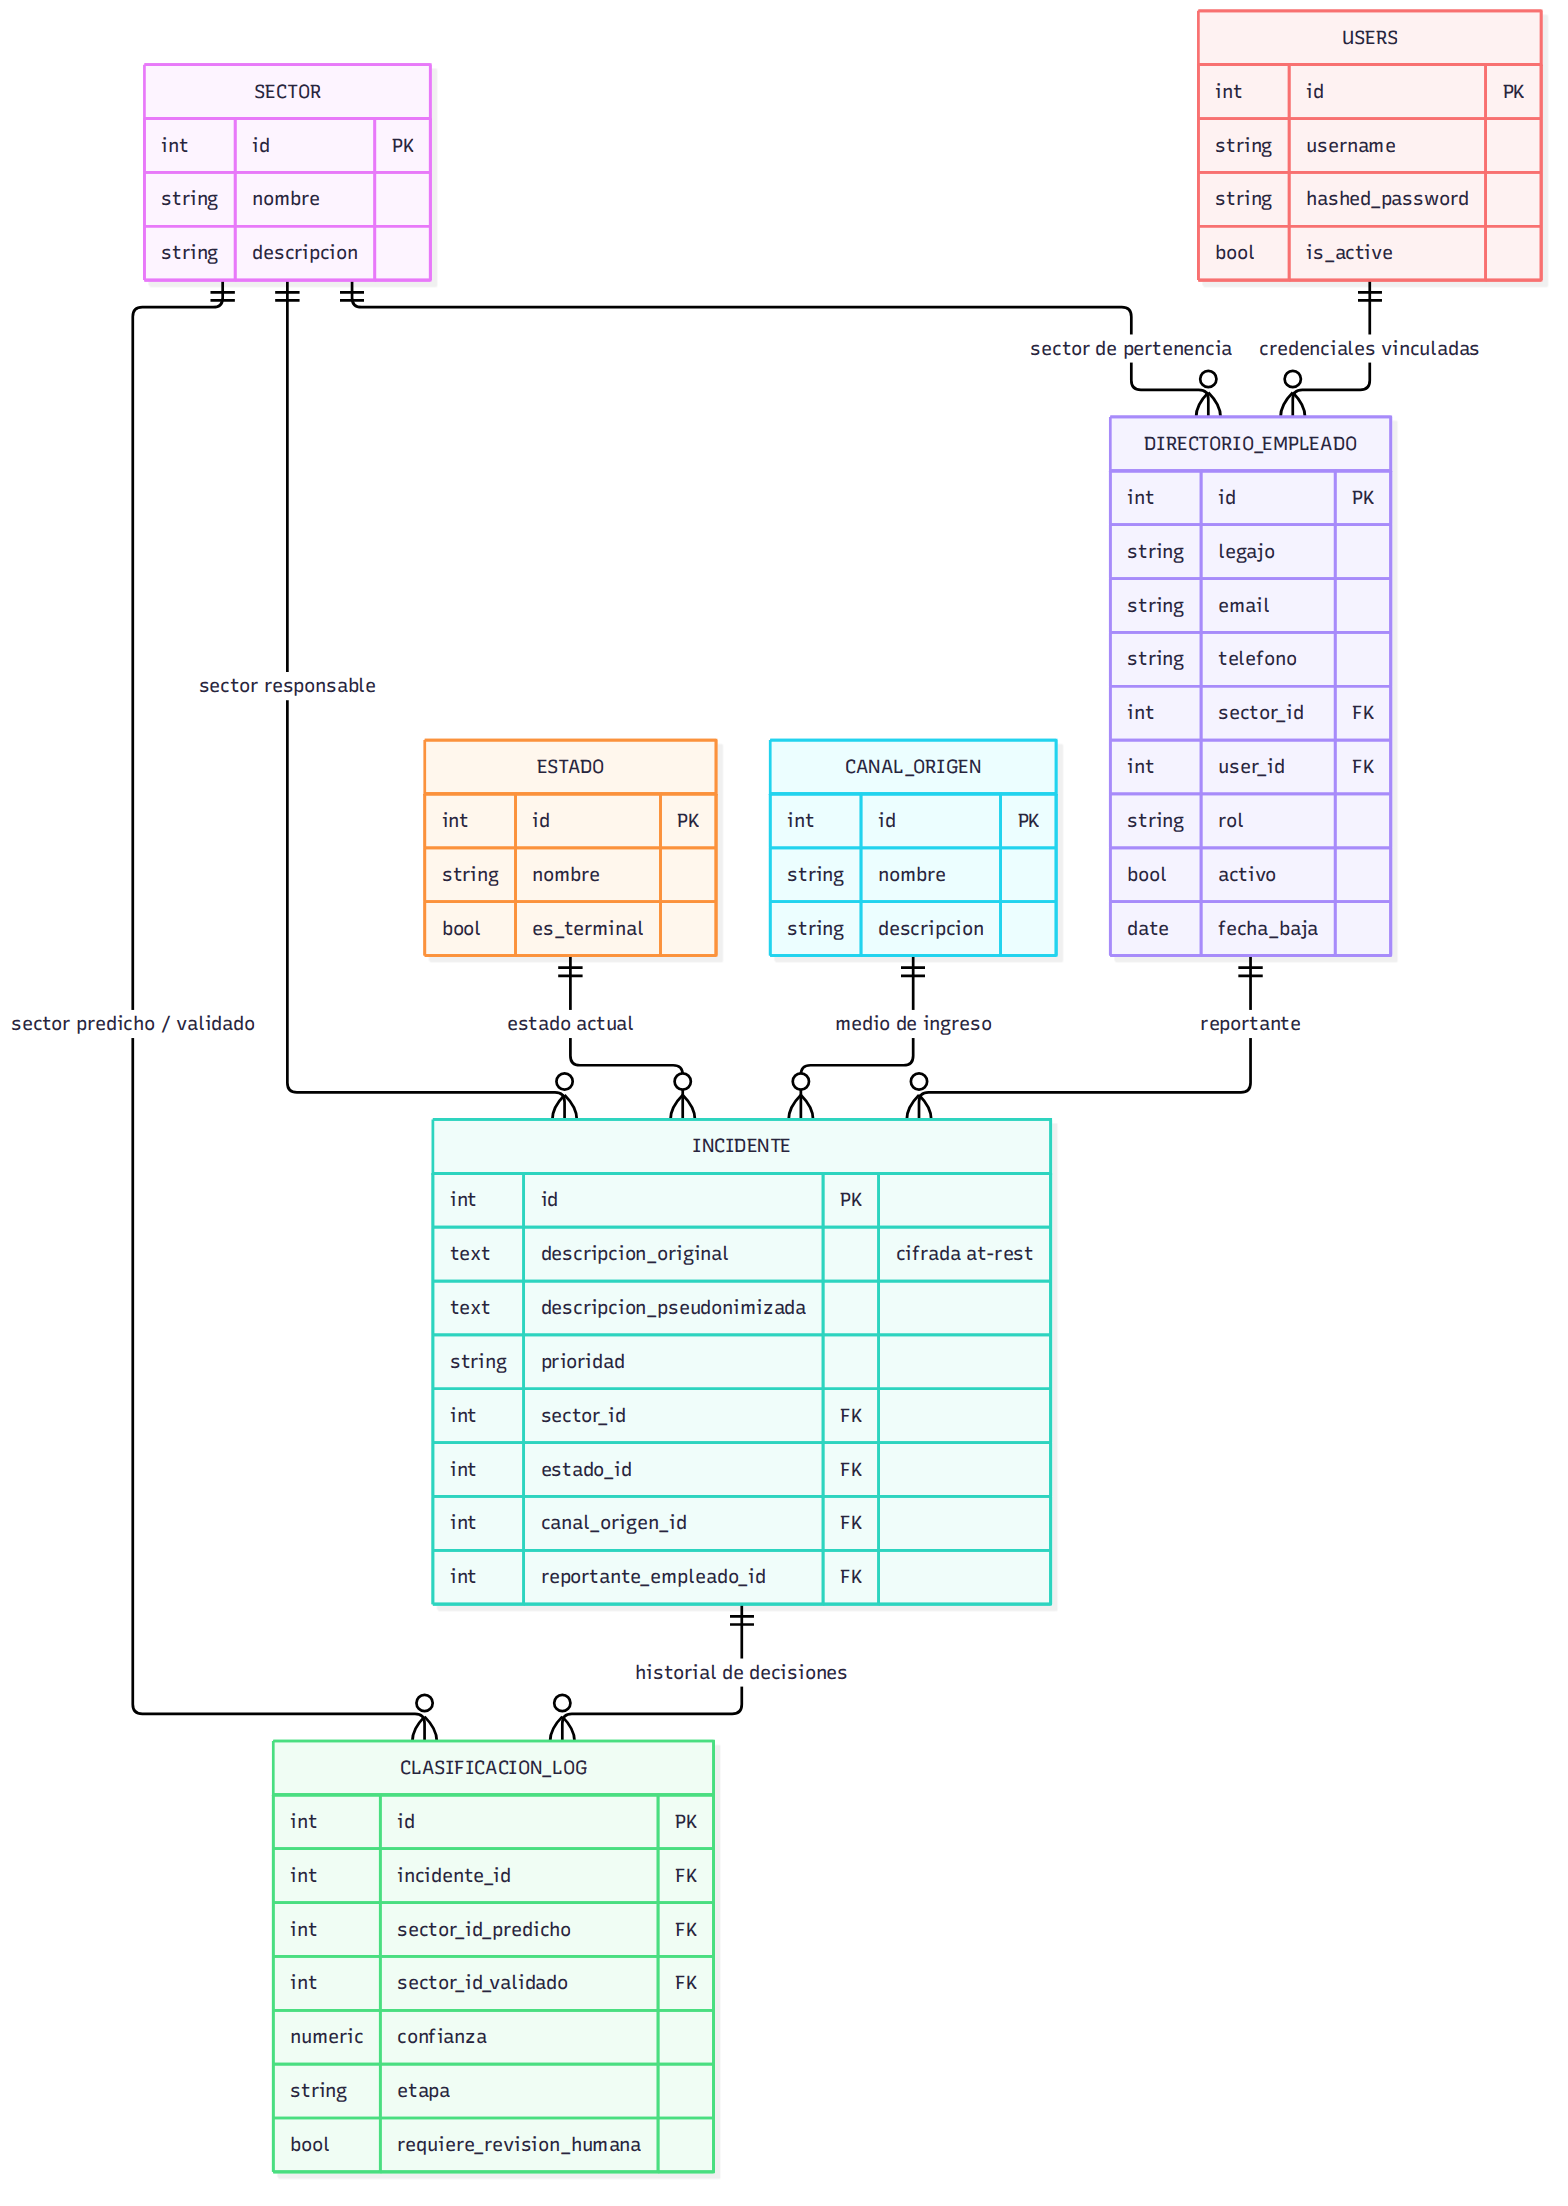
\includegraphics[width=0.85\textwidth]{er_modelo_datos}
\caption{Diagrama entidad-relación de las siete entidades principales del modelo de datos. El esquema completo se documenta en el Anexo~C.}
\label{fig:er_modelo_datos}
\end{figure}

\subsection{Contrato de la interfaz REST}

La interfaz de programacion de aplicaciones expuesta por el modulo Python sigue el estilo arquitectonico REST \parencite{Fielding2002_rest}, con representación de recursos mediante identificadores uniformes, uso semántico de los métodos HTTP estandar y comunicación sin estado del lado del servidor. La autenticacion se realiza mediante tokens JWT (JSON Web Tokens) firmados con HS256, validados en cada solicitud mediante el esquema OAuth2PasswordBearer de FastAPI. La Tabla~\ref{tab:api} sintetiza los principales puntos de entrada.

\begin{table}[htbp]
\centering
\caption{Puntos de entrada principales de la interfaz REST}
\label{tab:api}
\small
\begin{tabular}{@{}p{1.8cm} >{\raggedright\arraybackslash}p{5.2cm} p{1.8cm} >{\raggedright\arraybackslash}p{4.8cm}@{}}
\toprule
\textbf{Metodo} & \textbf{Ruta} & \textbf{Codigo} & \textbf{Funcion} \\
\midrule
\multicolumn{4}{@{}l}{\textbf{Autenticacion}} \\
POST & \texttt{/api/v1/auth/login}, \texttt{/refresh}, \texttt{/logout} & 200 OK & Inicio y renovacion de sesion y cierre de sesion de operadores. \\
GET & \texttt{/api/v1/auth/me} & 200 OK & Recupera el perfil del operador autenticado. \\
\midrule
\multicolumn{4}{@{}l}{\textbf{Incidentes}} \\
POST & \texttt{/api/v1/incidentes} & 201 Created & Crea un nuevo ticket y devuelve el identificador generado. \\
GET & \texttt{/api/v1/incidentes/\{id\}} & 200 OK & Recupera la información de un ticket por su identificador. \\
PATCH & \texttt{/api/v1/incidentes/\{id\}} & 200 OK & Actualiza los campos editables de un ticket. \\
\midrule
\multicolumn{4}{@{}l}{\textbf{Clasificaciones}} \\
GET & \texttt{/api/v1/clasificaciones/incidente/\{id\}} & 200 OK & Recupera la trazabilidad de la clasificación de un incidente. \\
GET & \texttt{/api/v1/clasificaciones/revision-pendiente} & 200 OK & Lista los casos derivados a revision humana. \\
PATCH & \texttt{/api/v1/clasificaciones/\{log\_id\}/validar} & 200 OK & Registra la categoría validada por el sector responsable. \\
\midrule
\multicolumn{4}{@{}l}{\textbf{Estadisticas}} \\
GET & \texttt{/api/v1/estadisticas/resumen}, \texttt{/tendencias} & 200 OK & Agregados y series temporales para el dashboard. \\
\midrule
\multicolumn{4}{@{}l}{\textbf{Salud}} \\
GET & \texttt{/health} y \texttt{/health/db} & 200 OK & Verificacion de salud del servicio para monitoreo externo. \\
\bottomrule
\end{tabular}
\par\smallskip
{\footnotesize\textit{Fuente:} elaboración propia.\par}
\end{table}

Los códigos de estado HTTP se utilizan conforme a su semántica original: 201 cuando un recurso se crea exitosamente, 200 cuando una consulta se atiende con éxito, 400 cuando los datos de entrada no validan el esquema esperado, 401 cuando la autenticacion falla, y 500 cuando ocurre un error interno no recuperable. La Tabla~\ref{tab:api} no es exhaustiva: reúne los grupos principales de puntos de entrada, mientras que el contrato completo de la interfaz ---que comprende la totalidad de las rutas expuestas--- se documenta en el Anexo~D, donde se incluye la especificación OpenAPI~3.1 que FastAPI genera automáticamente. La clasificación del incidente no se expone como punto de entrada independiente sino que se encuentra embebida dentro de la creación del incidente (POST \texttt{/api/v1/incidentes}): el clasificador híbrido se invoca internamente durante la creación y la respuesta incluye tanto el identificador del ticket como la categoría asignada y la confianza asociada.

\newpage
